\documentclass[FM,Proj]{tulthesis}

% tento dokument používá balíky specifické pro XeLaTeX a lze jej přeložit
% jen XeLaTeXem, nemáte-li instalována použitá (komerční) písma, změňte
% nebo vymažte příkazy \set...font na následujících řádcích

% Autor šablony: Pavel Satrapa: http://www.nti.tul.cz/~satrapa/vyuka/latex-tul/

% Autor komentářů, jejich překladů do EN, nastavení BibLaTeXu a aplikace ČSN ISO 690: Jan Koprnický
% http://www.fm.tul.cz/personal/jan.koprnicky

% ENGLISH EXPLANATION
% \documentclass[FM,Dis,EN,fonts,bw,twoside]{tulthesis} % black and white typing, dissertation thesis at FM, written in English with using of TUL Mono font, text is prepared to print on two sides of the paper
% this document uses packages specific for XeLaTeX and it is possible to 
% compile it by XeLaTeX only, if you haven't installed used (commercial) fonts
% change them or erase commands \set...font in following rows
% settings: FM (faculty: FS, FT, FP, EF, FA, FM, FZS a CXI), Dis (type of thesis: BP, DP, Teze, Autoref, Hab, SP, Proj), EN (written in English language), fonts (activation of TUL fonts), bw (black and white)

% Autor of the template tulthesis: Pavel Satrapa: http://www.nti.tul.cz/~satrapa/vyuka/latex-tul/

% Autor of several comments and their translation into English, BibLaTeX settings and CSN ISO 960 citation standard setting: Jan Koprnický
% http://www.fm.tul.cz/personal/jan.koprnicky

% poslední změna / last modification viz/see 00README-JK.txt

\newcommand{\verze}{2.0}

\usepackage{polyglossia}
\setdefaultlanguage{czech} % comment when English is preferred
%\setdefaultlanguage{english} % comment when Czech is preferred


\usepackage{makeidx}
\makeindex

\usepackage{xunicode}
\usepackage{xltxtra}

\usepackage{float}

% příkazy specifické pro tento dokument / specific commands for this document
\newcommand{\argument}[1]{{\ttfamily\color{\tulcolor}#1}}
\newcommand{\argumentindex}[1]{\argument{#1}\index{#1}}
\newcommand{\prostredi}[1]{\argumentindex{#1}}
\newcommand{\prikazneindex}[1]{\argument{\textbackslash #1}}
\newcommand{\prikaz}[1]{\prikazneindex{#1}\index{#1@\textbackslash #1}}
\newenvironment{myquote}{\begin{list}{}{\setlength\leftmargin\parindent}\item[]}{\end{list}}
\newenvironment{listing}{\begin{myquote}\color{\tulcolor}}{\end{myquote}}
\sloppy

% deklarace pro titulní stránku / title page declaration
\TULtitle{Filtr nevhodného textového obsahu pro herní server s využitím strojového
učení}{}
\TULauthor{ Mikhail Belov, German Semin}

% pro bakalářské, diplomové a disertační práce / for bachelor, master theses and dissertation
\TULprogramme{N2612}{Elektrotechnika a informatika}{Electrical engineering and informatics}
\TULbranch{1802T007}{Informační technologie}{Information technology}
%\TULbranch{1802T008}{Nějaký jiný obor}{Some other branch}
\TULsupervisor{Ing. Lukáš Matějů, Ph.D}
%\TULconsultant{doc. RNDr. Pavel Satrapa, Ph.D.}
%\TULconsultant{doc. RNDr. Druhý Konzultant, Ph.D.}
%\TULconsultant{doc. RNDr. Třetí Konzultant, Ph.D.}
\TULyear{2025}

% pro habilitační práce / habilitation thesis
%\TULbranch{}{Technická kybernetika}{Technical cybernetics}
%\TULyear{2022}

% Použití bibLateXu, pracuje s ISO stylem
% BibLaTeX settings, works with ISO style
\usepackage[ 
    backend=biber
     % ,style=iso-authoryear % styl vyžaduje FZS TUL , místo příkazu \cite{} je potřeba využít \parencite{} (sazba kulatých závorek) / style required by FZS TUL use \parencite{} instead of \cite{}
    ,style=iso-numeric
    %,style=numeric
    %,sortlocale=cs_CZ
    ,sorting=nyt %seřazeno jméno, rok, titul
    ,autolang=other
    ,bibencoding=UTF8
    %,urldate=edtf
    ,maxcitenames=2 %maximum v textu citovaných jmen
    ,maxbibnames=3 %maximum v seznamu vyjmenovaných autorů
    ]{biblatex}
\addbibresource{refTULTHESIS.bib}% vložení seznamu literárních zdrojů v bib formátu / input of references in bib format

% Úprava iso-numeric.bbx v souladu s požadavky TUL hranaté závorky v číslovaném seznamu / Modification of iso-numeric.bbx in accordance with TUL requirements of square brackets in a numbered list
\DeclareFieldFormat{labelnumberwidth}{\mkbibbrackets{#1}}

% Formátování podle pokynů FZS, při využití stylu iso-authoryear, čárka mezi jmény a poslední jméno se spojkou a / special requirements of FZS TUL 
\DeclareDelimFormat{multinamedelim}{\addcomma\space}

\DeclareDelimFormat{finalnamedelim}{%
  \ifnumgreater{\value{liststop}}{2}{\finalandcomma}{}%
  \addspace\bibstring{and}\space}

\DeclareNameAlias{author}{family-given/given-family} 
%%%%%%%%%%%%%%%%%%%%%%%%%%

\usepackage{csquotes} %užití biblatexu hlasí warnings, důvodem může být použití českých uvozovek v citacích! / solving of problems with Czech quotations
\urlstyle{same} %sazba url odkazů stejným fontem jako ostatní text, řešení problémů v zalamování hypertextových odkazů v citacích / url in references setting into the same form as text 

\usepackage{listings} %package for sourcode typesetting
%řešení problémů češtiny např. při sazbě zdrojových kódů / czech special characters in sourcecode typesetting
\makeatletter
\lst@InputCatcodes
\def\lst@DefEC{%
 \lst@CCECUse \lst@ProcessLetter
  ^^80^^81^^82^^83^^84^^85^^86^^87^^88^^89^^8a^^8b^^8c^^8d^^8e^^8f%
  ^^90^^91^^92^^93^^94^^95^^96^^97^^98^^99^^9a^^9b^^9c^^9d^^9e^^9f%
  ^^a0^^a1^^a2^^a3^^a4^^a5^^a6^^a7^^a8^^a9^^aa^^ab^^ac^^ad^^ae^^af%
  ^^b0^^b1^^b2^^b3^^b4^^b5^^b6^^b7^^b8^^b9^^ba^^bb^^bc^^bd^^be^^bf%
  ^^c0^^c1^^c2^^c3^^c4^^c5^^c6^^c7^^c8^^c9^^ca^^cb^^cc^^cd^^ce^^cf%
  ^^d0^^d1^^d2^^d3^^d4^^d5^^d6^^d7^^d8^^d9^^da^^db^^dc^^dd^^de^^df%
  ^^e0^^e1^^e2^^e3^^e4^^e5^^e6^^e7^^e8^^e9^^ea^^eb^^ec^^ed^^ee^^ef%
  ^^f0^^f1^^f2^^f3^^f4^^f5^^f6^^f7^^f8^^f9^^fa^^fb^^fc^^fd^^fe^^ff%
% české znaky
  ^^^^010c^^^^010d^^^^010e^^^^010f^^^^011a^^^^011b^^^^0147^^^^0148%
  ^^^^0158^^^^0159^^^^0160^^^^0161^^^^0164^^^^0165%
  ^^^^016e^^^^016f^^^^017d^^^^017e%
  ^^00}
\lst@RestoreCatcodes
\makeatother

\begin{document}

\ThesisStart{male}
%\ThesisStart{zadani-a-prohlaseni.pdf}

\begin{abstractCZ}
Tento semestrální projekt se zabývá vývojem Discord bota, který automaticky detekuje toxický obsah v textových zprávách na serveru. Cílem je analyzovat a porovnat čtyři různé metody detekce toxického obsahu – od jednoduchých slovníkových filtrů a regulárních výrazů po moderní přístupy využívající strojové učení a velké jazykové modely (LLM). Jednotlivé metody jsou hodnoceny podle přesnosti, rychlosti zpracování a provozních nákladů. Nejlepší řešení je následně implementováno v rámci Discord bota, který upozorní lidského moderátora na podezřelé zprávy.

\end{abstractCZ}

\begin{keywordsCZ}Discord bot, Toxický obsah, Detekce nevhodných zpráv, Strojové učení, Velké jazykové modely, Slovníkové filtry, Regulární výrazy, Moderace, Online komunikace
\end{keywordsCZ}

\vspace{2cm}

\begin{abstractEN}

This semester project focuses on the development of a Discord bot that automatically detects toxic content in text messages on the server. The aim is to analyze and compare four different methods of toxicity detection—from simple dictionary-based filters and regular expressions to modern machine learning approaches, including large language models (LLMs). The methods are evaluated based on accuracy, processing speed, and operational costs. The best-performing solution is implemented in the Discord bot, which alerts a human moderator to suspicious messages.
rts a human moderator to suspicious messages.
\end{abstractEN}

\begin{keywordsEN}
Discord bot, Toxic content, Detection of inappropriate messages, Machine learning, Large language models, Dictionary filters, Regular expressions, Moderation ,Online communication
\end{keywordsEN}

\clearpage

\begin{acknowledgement}
Rádi bychom poděkovali panu doktorovi Lukáši Matějů za jeho trpělivost, odborné vedení a cenné rady, které nám pomohly úspěšně dokončit tento semestrální projekt. Jeho profesionální přístup a vstřícnost byly pro nás velkou oporou během celého procesu vývoje.

Zvláštní poděkování patří také administrátorům komunitních serverů „Kill or Die“ (DayZ) a „nullhaven“ (Minecraft) za jejich ochotu spolupracovat a poskytnout přístup k datům nezbytným pro trénování a testování našeho modelu.

Bez jejich pomoci by realizace tohoto projektu nebyla možná.
\end{acknowledgement}

\tableofcontents

\clearpage

\begin{abbrList}
\textbf{API} & Application Programming Interface / Rozhraní pro programování aplikací \\
\textbf{CSV} & Comma-Separated Values / Formát pro ukládání dat oddělených čárkami \\
\textbf{HTTP} & HyperText Transfer Protocol / Protokol pro přenos hypertextu \\
\textbf{IM} & Instant Messaging / Okamžité zprávy \\
\textbf{JSON} & JavaScript Object Notation / Datový formát pro výměnu informací \\
\textbf{LLM} & Large Language Model / Velký jazykový model \\
\textbf{NLP} & Natural Language Processing / Zpracování přirozeného jazyka \\
\textbf{Regex} & Regular Expressions / Regulární výrazy \\
\textbf{ruBERT} & Russian Bidirectional Encoder Representations from Transformers \\
\textbf{SDK} & Software Development Kit / Sada nástrojů pro vývojáře \\
\textbf{UI} & User Interface / Uživatelské rozhraní \\
\textbf{VRAM} & Video Random Access Memory / Grafická operační paměť \\
\end{abbrList}

\chapter{Úvod}
\section{Seznámení s problémem}\label{deklarace}

Při správě dvou herních serverů — Minecraft serveru “nullhaven” a roleplay serveru “Kill or Die: Stalker RP” pro hru DayZ — jsme s kolegou narazili na vážný problém: nízká účinnost automatické filtrace zpráv v prostředí Discord. Ačkoli Discord nabízí základní moderovací nástroje, ve skutečnosti buď přehnaně omezují běžnou komunikaci, nebo naopak nedokážou zachytit toxický a závadný obsah.

Tento problém přitom není jen otázkou pohodlí komunity. Podmínky služby Discord jasně stanovují, že nevhodné zprávy mohou vést k trvalému zablokování celého serveru — a to i v případě, že se zprávy objevily bez vědomí administrace. Jinými slovy, bez aktivního a externího dohledu je možné, že chování jednotlivců ohrozí existenci celého projektu.

V případě komunitních herních serverů, které navíc nabízejí placený obsah nebo herní výhody, představuje takové zablokování přímé finanční riziko. I krátkodobé pozastavení provozu může vést ke ztrátám způsobeným výpadkem hráčů, přerušením prodejů a narušením reputace.

Cílem tohoto projektu je proto vytvořit inteligentní systém filtrace zpráv, který bude v reálném čase analyzovat obsah a upozorňovat na potenciálně problematické příspěvky. Tímto způsobem lze odlehčit práci moderátorům, kteří by jinak museli ručně kontrolovat tisíce zpráv denně. Zároveň se tím výrazně sníží riziko porušení pravidel Discordu a vznikne tak první krok k automatizované moderaci online komunikace, která je klíčová pro dlouhodobou udržitelnost herních komunit.

\section{Související práce}

V řadě studií byla zkoumána problematika automatického rozpoznávání toxických a urážlivých zpráv na sociálních sítích. Ve studii Smetanin S. I. (2020) \cite{smetanin2020toxic} byly pro ruský jazyk testovány moderní jazykové modely (Multilingual BERT, ruBERT \cite{deeppavlov2020rubertcasebased}, Multilingual USE) na otevřeném Kaggle datasetu \cite{blackmoon2019russiantoxiccomments}, přičemž nejlepších výsledků bylo dosaženo s~doinstruovaným modelem ruBERT (F1 = 92{,}2~\%). Ve~výzkumu Prabowo a kol. (2019) \cite{prabowo2019identifyhatespeech} byl pro indonéský Twitter navržen hierarchický multi-label přístup, který umožnil nejen detekovat přítomnost toxicity, ale i klasifikovat zprávy podle kategorií a cílových skupin, což vedlo k flexibilnější a detailnější analýze.

Na rozdíl od těchto prací je tento projekt zaměřen na praktickou úlohu automatické filtrace toxického obsahu v prostředí herních serverů Discord, kde zprávy často obsahují herní slang a neformální výrazy. V rámci projektu byly porovnávány různé metody -- od regulárních výrazů po moderní jazykové modely, přičemž zvláštní důraz je kladen na do-učení modelu ruBERT na reálných Discord zprávách za účelem zvýšení přesnosti detekce toxicity v konkrétním online prostředí. Na rozdíl od hierarchických či multi-label přístupů je zde implementována efektivní binární filtrace optimalizovaná na rychlost a jednoduchou integraci do infrastruktury herních služeb.

\section{Návrh řešení a přístup}\label{deklarace} 
Po analýze situace jsme se rozhodli navrhnout vlastní systém pro automatické rozpoznávání nevhodných zpráv. Vzhledem k tomu, že jde o specifickou jazykovou oblast a zároveň o prostředí, kde hráči komunikují neformálně , běžné metody filtrace založené pouze na klíčových slovech se ukázaly jako nedostačující.

Rozhodli jsme se porovnat pět různých přístupů k detekci toxického obsahu:

\begin{enumerate}
    \item Jednoduchá filtrace pomocí regulárních výrazů — základní slovník zakázaných slov.
    \item Použití předtrénovaného jazykového modelu — například ruBERT \cite{kuratov2019adaptationdeepbidirectionalmultilingual}, který byl trénován přímo pro ruský jazyk.
    \item Vlastní model natrénovaný na reálném datasetu z Discordu — přizpůsobený specifickému kontextu herní komunity.
    \item Velký jazykový model (LLM) — například Groq nasazený s modelem jako LLaMA, který dokáže analyzovat význam zpráv v širším kontextu a poskytnout velmi přesné hodnocení i u složitějších struktur.
    \item Groq jako inference platforma — umožňuje extrémně rychlé zpracování požadavků s nízkou latencí, což je výhodné pro reálné nasazení v prostředí s vysokou zátěží, jako jsou herní komunity.
\end{enumerate}

\chapter{Příprava datasetu a možné přístupy k jeho využití}
Tato kapitola se zaměřuje na proces přípravy dat pro detekci toxických zpráv ve vybraném prostředí. Vysvětlujeme zde metodiku sběru dat z Discord serverů, jejich následné čištění a anotaci. Pozornost je věnována i jazykové specifice, protože značná část zpráv je v ruském jazyce a bylo tedy nutné řešit otázku práce s cyrilicí. V další části kapitoly popisujeme různé přístupy, které jsme zvažovali pro klasifikaci zpráv – od jednoduchých metod (např. regulární výrazy) až po pokročilé přístupy využívající neuronové sítě a velké jazykové modely. Výsledkem této přípravné fáze je sestavení robustního datasetu, který slouží jako základ pro experimentální testování jednotlivých řešení.
\section{Sběr a požadavky na dataset}\label{deklarace}
Zásadním krokem před samotným testováním bylo získání kvalitního datasetu reálných zpráv z Discordu. Sběr probíhal prostřednictvím vlastního skriptu, který využíval přímý přístup k Discord API bez nutnosti použití bota. Získaná data byla poté uložena ve strukturované podobě (uživatel + zpráva + štítek).

Hlavní požadavky na dataset:

\begin{itemize}
    \item Jazyk dat: ruština – většina zpráv na našich serverech je psána cyrilicí.
    \item Reálné zprávy od hráčů – zprávy byly sbírány z veřejných i soukromých kanálů.
    \item Vyváženost dat – dataset obsahoval přibližně stejné množství "neutrálních" a "toxických" zpráv.
    \item Ruční anotace – každá zpráva byla označena štítkem 0 (v pořádku) nebo 1 (nevhodná/toxická).
\end{itemize}
\section{Sběr dat z Discordu}\label{deklarace}

Prvním krokem při realizaci projektu bylo získání dostatečně velkého a reprezentativního datasetu zpráv, na kterém bylo možné trénovat klasifikační model. Vzhledem k tomu, že oficiální Discord API neumožňuje snadný přístup k historii zpráv bez použití bota, bylo nutné zvolit alternativní přístup.

Byl vytvořen vlastní Python skript, který přímo komunikuje s rozhraním Discord API pomocí HTTP požadavků přes knihovnu requests. Tento skript postupně stahuje historii zpráv z určeného kanálu pomocí parametrů limit a before, čímž umožňuje iterativní procházení celé historie.

Pro rozšíření množiny trénovacích dat jsme navíc dataset doplnili o další zprávy z veřejně dostupného datasetu publikovaného na platformě Kaggle uživatelem blackmoon (Anatoliy Belchikov) \cite{blackmoon2019russiantoxiccomments}. Tato data byla sloučena s naším vlastním korpusem, což umožnilo získat ještě robustnější a vyváženější soubor pro trénink modelu.

Klíčové body implementace:

\begin{itemize}
    \item Autentizace pomocí uživatelského tokenu: skript používá ručně získaný autorizovací token (nikoliv bota), což umožňuje přístup k datům bez nutnosti vytvářet a registrovat aplikaci.
    \item Iterativní načítání zpráv: díky parametru before je možné postupně stahovat starší zprávy, dokud se nevyčerpá celá historie.
    \item Uložení zpráv ve formátu CSV nebo Excel: zprávy byly ukládány společně s uživatelským jménem a připraveným polem pro ruční anotaci (label), které následně sloužilo jako vstupní data pro trénink modelu.
\end{itemize}
Příklad výstupního formátu:
\begin{verbatim}
username,message,label
meteoru,privet vsem,0
rouus3,blja idi nahui,1
\end{verbatim}
Zvláštní pozornost byla věnována:

\begin{itemize}
    \item Odstranění prázdných zpráv, příkazů bota a systémových hlášek
    \item Zajištění toho, aby každá zpráva byla na samostatném řádku
    \item Doplnění labelu 0 (neškodné) nebo 1 (toxické) pro účely učení s učitelem
\end{itemize}

Tímto způsobem se podařilo nashromáždit více než 10 000 reálných i syntetických zpráv, což vytvořilo solidní základ pro následné modelování.

\section{Základní metriky datasetu}
\label{sec:dataset-metrics}

\begin{table}[H]
\centering
\caption{Rozložení tříd v trénovací a testovací sadě}
\begin{tabular}{lcc}
\hline
\textbf{Sada} & \textbf{Netoxické zprávy (0)} & \textbf{Toxické zprávy (1)} \\
\hline
Trénovací     & 11\,665 & 7\,864 \\
Testovací     & 2\,921 & 1\,962 \\
\hline
Celkem        & 14\,586 & 9\,826 \\
\hline
\end{tabular}
\label{tab:dataset-split}
\end{table}

\begin{itemize}
    \item \textbf{Celkový počet zpráv:} 24\,412
    \item \textbf{Počet toxických zpráv:} 9\,826 (\textasciitilde 40~\%)
    \item \textbf{Počet netoxických zpráv:} 14\,586 (\textasciitilde 60~\%)
    \item \textbf{Rozsah délky zprávy:} 9 až 7404 znaků
\end{itemize}

\section{Klasifikační metriky a interpretace výsledků}

Pro hodnocení kvality detekce toxicity v různých případech byly použity čtyři základní klasifikační metriky:

\begin{itemize}
    \item \textbf{Accuracy (přesnost)} – podíl správně klasifikovaných zpráv vůči celkovému počtu.
    \item \textbf{Recall (záchyt)} – měří, kolik zpráv dané třídy bylo správně rozpoznáno. U toxicity je klíčový recall pro třídu „toxická“, protože určujeme, kolik nevhodného obsahu bylo zachyceno.
    \item \textbf{F1 skóre (F1-score)} – harmonický průměr mezi recall a přesností; slouží jako vyvážený ukazatel výkonnosti modelu. Používáme to pro porovnání různých přístupů.
    \item \textbf{Support (podpora)} – počet zpráv dané třídy v testovací sadě. Vyjadřuje, na jak velkém vzorku byly metriky spočítány.
\end{itemize}

Tyto metriky umožňují objektivní porovnání jednotlivých modelů a byly použity ve všech experimentech uvedených v této práci.

\chapter{Experimenty a vyhodnocení výsledků}
Tato kapitola se věnuje testování navržených metod na reálných datech. Porovnáváme zde výkonnost jednotlivých řešení pomocí standardních klasifikačních metrik (precision, recall, F1-score) a zohledňujeme také jejich vhodnost pro praktické nasazení. Výsledky jsou prezentovány v tabulkách a doplněny interpretací.

\section{ Metoda regulárních výrazů}\label{deklarace}
Při prvním návrhu filtru jsme se rozhodli využít regulární výrazy, protože se osvědčily jako jednoduchý a přitom flexibilní způsob, jak zachytit různé varianty nežádoucích slov. Z chatovacích dat bylo jasné, že slova, která nechceme na serveru vidět, se často vyskytují v kreativních podobách: uživatelé nahrazují některá písmena podobnými znaky, vkládají čísla, mezery nebo speciální znaky, aby automatický filtr obešli.

Například běžné slovo jako „hlupák“ může být v chatu zapsáno jako „h1upak“, „hlup@k“, „h.l.u.p.a.k“, „h|upak“, nebo „h l u p a k“. Pokud bychom se spoléhali jen na přesné shody, většina těchto variant by filtrem snadno prošla. Regulární výrazy však umožňují vytvořit vzor, který zachytí všechny tyto úpravy najednou.

Typický vzor pro slovo „hlupák“ může vypadat například takto:
\begin{verbatim}
import re

pattern = r"h[l1|][uú][p][áa@][k]"
text = "h|upak"
if re.search(pattern, text.lower()):
    print("Nalezeno nevhodné slovo.")
\end{verbatim}
V tomto vzoru:
\begin{itemize}
    \item „l“ je možné nahradit za „l“, „1“ nebo „|“
    \item „u“ lze napsat jako „u“ nebo „ú“
    \item „á“ může být „á“, „a“ nebo „@“
\end{itemize}
Stejný princip jsme použili i pro další slova, například „trol“ (`t[r][o0][l1]`) nebo „blázen“ (`b[l1][áa][z2][eě][n]`). Vzory jsme vytvářeli postupně podle toho, jaké úpravy slov se v chatu skutečně objevily.

Výhodou tohoto přístupu je, že vzory lze snadno upravovat a rozšiřovat, když se objeví nová varianta nežádoucího slova, a samotné filtrování je velmi rychlé. Problém ale nastává v případech, kdy se část vzoru náhodou objeví v úplně neškodném slově. Tento jev je známý jako „Scunthorpe problém“ – tedy situace, kdy filtr označí běžné slovo za nevhodné jen proto, že obsahuje sekvenci znaků podobnou zakázanému výrazu.

Během testování jsme narazili na několik takových případů – například pokud se vzor trefil do části neškodného příjmení nebo názvu. I proto jsme začali uvažovat o metodách, které umí zohlednit význam celé věty a nejen jednotlivá písmena nebo slova.
\section{ Klasifikace zpráv pomocí jazykového modelu ruBERT a následné do-učení}\label{deklarace}
Po testování filtru založeného na regulárních výrazech se ukázalo, že tento přístup má své limity, zejména v situacích, kdy je nevhodnost obsahu dána spíše významem celé věty, než přítomností konkrétního slova. Proto jsme jako další krok zvolili využití moderního jazykového modelu ruBERT, postaveného na architektuře BERT \cite{devlin2018bert}.

\textbf{Příprava dat}

Nejdříve byl sestaven datový korpus, který obsahoval reálné zprávy ze sledovaného herního serveru. Soubor zpráv zahrnoval jak běžnou komunikaci, tak i zprávy s projevy nevhodného nebo konfliktního chování. Každá zpráva byla ručně anotována – označili jsme ji jako „přijatelnou“ nebo „nepřijatelnou“. Při této práci jsme dbali na to, aby anotace odpovídala nejen obecným pravidlům slušné komunikace, ale i specifikům herní komunity: různé vtipy, narážky, slang a herní fráze. Použitý dataset byl složen z veřejně dostupného korpusu z platformy Kaggle, který obsahuje 14,412 komentářů (z toho 4,826 bylo označeno jako toxické a 9,586 jako netoxické), a dále z našeho vlastního datasetu o velikosti 10,000 zpráv, kde bylo 5,000 zpráv ručně označeno jako toxické a 5,000 jako netoxické.

Pro zvýšení kvality a spolehlivosti učení byly zprávy předzpracovány – odstranily se technické znaky, sjednotil se zápis písmen a nadbytečné mezery. Takto připravená data byla rozdělena na dvě části: 80\,\% zpráv bylo použito pro trénování (trénovací sada) a zbývajících 20\,\% bylo vyhrazeno pro testování (testovací sada). Toto rozdělení umožnilo objektivně ověřit schopnosti modelu na zprávách, které nikdy „neviděl“ během učení.

\textbf{Použití předtrénovaného modelu}

První experimenty proběhly s použitím základní, veřejně dostupné předtrénované verze ruBERT (DeepPavlov/rubert-base-cased). Model dostal na vstup jednotlivé zprávy a vrátil pravděpodobnost, že obsahují nevhodný obsah. Tato strategie přinesla dobré výsledky pro zprávy s jasnými projevy toxicity nebo jednoznačnými urážkami.

Ukázalo se však, že v některých případech model označoval i nevinné vtipy nebo herní slang za nevhodné, případně naopak přehlédl rafinovanější formy toxického chování, například ironii, kombinace více jazyků, nebo nové kreativní výrazy. Z těchto důvodů bylo potřeba model lépe přizpůsobit specifickému prostředí herního chatu.

\textbf{Do-učení modelu na vlastních datech}

Proto jsme přistoupili k do-učení (fine-tuning) modelu ruBERT na našem vlastním korpusu. Pro tento krok jsme využili knihovnu Huggingface Transformers a PyTorch, které umožňují efektivní trénink velkých jazykových modelů. Model byl do-učován v režimu klasifikace textu na dvě třídy („přijatelné“, „nepřijatelné“), přičemž vstupem byly připravené a anotované zprávy z našeho datasetu.

Při do-učení jsme použili běžné trénovací parametry: maximální délka zprávy 64 tokenů, optimalizátor AdamW, learning rate 2e-5, batch size 16 a počet epoch mezi 3 a 5 (počet epoch byl volen podle výsledků na testovací sadě tak, aby nedošlo k přeučení modelu).

V průběhu tréninku jsme sledovali metriky přesnosti, preciznosti, recall a F1-score na testovací sadě, což umožnilo optimalizovat výkon modelu právě v našem prostředí.

\section{ Využití jazykového modelu LLaMA3 prostřednictvím API Groq pro automatickou moderaci uživatelských zpráv
}\label{deklarace}
Po úspěšném nasazení a přizpůsobení modelu ruBERT specifikům herního chatu vznikla potřeba otestovat univerzálnější a flexibilnější řešení, které by bylo schopno zachytit i složitější formy toxicity — například skryté urážky, nepřímou agresi nebo jiné formy porušování pravidel, které nejsou vždy explicitně vyjádřené. Za tímto účelem byl implementován jazykový model z rodiny LLaMA3 \cite{grattafiori2024llama3herdmodels}, dostupný prostřednictvím vzdáleného API platformy Groq.

\textbf{Důvody, proč jsme se rozhodli neprovozovat LLM lokálně}

\begin{itemize}
    \item V počáteční fázi byla testována možnost lokálního spuštění modelu "gemma3:4b" pomocí nástroje Ollama. Ačkoli bylo toto řešení teoreticky proveditelné, v praxi se ukázalo jako neefektivní kvůli následujícím omezením:
    \item Hardwarová náročnost. Model s 4 miliardami parametrů vyžaduje výkonný grafický akcelerátor s dostatečně velkou pamětí (alespoň 8–12 GB VRAM), což není v běžném prostředí dostupné a v cloudových službách jako Google Colab je navíc značně omezené.
    \item Nízká stabilita a náročná údržba. Spuštění Ollamy vyžaduje instalaci pomocného démona, konfiguraci síťových portů, správu závislostí a pravidelný dohled, což neodpovídá požadavkům na stabilní a snadno udržovatelný provoz.
    \item Omezená škálovatelnost. Při zvýšené zátěži (např. vyšším počtu příchozích zpráv) rychle narážíme na limity výkonu a horizontální škálování vyžaduje výrazné investice do infrastruktury.
\end{itemize}
    
Na základě těchto faktorů bylo rozhodnuto upustit od lokální varianty a přejít na cloudové řešení formou API.

\textbf{Volba Groq jako platformy pro využití LLM}

Platforma "Groq" byla zvolena jako externí řešení pro integraci LLM díky souhrnu technických, ekonomických a praktických výhod:

\begin{itemize}
    \item Přístup k moderním modelům. Groq poskytuje vysoce výkonný přístup k modelům rodiny LLaMA3, včetně nejnovějších verzí s podporou režimu `json mode` a širokého kontextového okna.
    \item Ekonomická efektivita. Bezplatný tarif platformy umožňuje až 14 400 požadavků denně, což více než pokrývá náš aktuální denní provoz (přibližně 3 000–4 000 zpráv denně).
    \item Podpora strukturovaných výstupů. Groq umožňuje přesně definovat formát odpovědi, což je zásadní pro snadnou integraci s automatickými filtry a dalšími systémy.
\end{itemize}
    
Tímto způsobem jsme získali spolehlivou a snadno replikovatelnou infrastrukturu pro analýzu zpráv v reálném čase, bez potřeby správy vlastního výpočetního prostředí.

\textbf{Formulace a význam systémového promptu}

Zásadním prvkem při nastavování chování jazykového modelu je tzv. "systémový prompt" – textová instrukce, která určuje, jak má model interpretovat a klasifikovat vstupní zprávy.

Pro tento konkrétní případ jsme použili následující prompt (v anglickém jazyce, jak vyžaduje model):
\begin{verbatim}
<task>
You are a professional content moderation system.
Evaluate user messages for toxicity. Your goal is to classify
each message as either  "toxic" or "normal".

A message is "toxic" if it contains any of the following:
- Hate speech (e.g., racism, sexism, homophobia)
- Threats or incitement to violence
- Harassment or targeted abuse
- Sexually explicit or obscene content
- Severe profanity or slurs
- Graphic self-harm or suicide encouragement

A message is "normal" if it contains none of the above.

If a message is toxic, you must also provide a brief reason for the
classification, using one of the following categories:
"hate speech", "threat", "harassment", "sexual content", 
"profanity", or "self-harm".

For ambiguous or borderline cases, choose "normal" unless
clear evidence of toxicity is present.

Consistency and accuracy are critical. Do not guess or interpret
intent—classify only the content provided.

Classify each message exactly as instructed, with no explanation, 
markdown, or extra text.
</task>

<input>
You will receive a raw user message as the next message. Treat it as-is.
</input>

<output>
Respond in **exactly** one of the following JSON formats, with no extra
whitespace or characters.
If the message is toxic:
{
  "type": "toxic",
  "reason": "CATEGORY"
}

If the message is normal:
{
  "type": "normal"
}
</output>
\end{verbatim}
Hlavní výhodou je skutečnost, že model nyní musí kromě označení toxicity také uvést důvod, proč bylo dané sdělení klasifikováno jako nevhodné, a to jedním z následujících předdefinovaných důvodů: `hate speech`, `threat`, `harassment`, `sexual content`, `profanity`, `self-harm`.

Tato úprava přinesla několik klíčových výhod:

\begin{itemize}
    \item Zvýšenou informační hodnotu výsledků – umožňuje přesněji sledovat typy nevhodného chování.
    \item Lepší interpretovatelnost modelu – každý výstup lze přímo vysvětlit na základě dané kategorie.
    \item Možnost další analytiky – výstupy mohou být statisticky zpracovávány a využívány např. při vytváření přehledů nebo reportů o činnosti moderace.
\end{itemize}
\textbf{Způsob integrace a použití API}

Každá příchozí zpráva od uživatele byla zpracována podle následujícího schématu:

 Vytvořil se požadavek na API Groq, který obsahoval:
    \begin{itemize}
        \item systémové sdělení s výše uvedeným promptem, označené rolí `system`;
        \item Uživatelskou zprávu označenou jako role `user`.
    \end{itemize}
 Model následně vracel odpověď ve striktním formátu JSON, např. :
\begin{verbatim}
<task>

{
  "type": "normal"
}

nebo

{
  "type": "toxic",
  "reason": "profanity"
}
\end{verbatim}
Získané výsledky byly automaticky zpracovávány a ukládány do databáze. Zprávy označené jako `toxic` byly dále směrovány do moderačního systému a zpracovany člověkem.

Díky přesně definovanému formátu výstupu a explicitní klasifikaci důvodu toxicity se systém ukázal jako stabilní, přehledný a snadno rozšiřitelný. Kromě samotné moderace se výstupy z modelu staly cenným zdrojem pro analýzu chování uživatelů a ladění komunikačních pravidel na sledovaném serveru.

\begin{table}[H]
\centering
\caption{Výsledky klasifikace zpráv (Regex)}
\begin{tabular}{lcccc}
\hline
\textbf{Třída} & \textbf{Přesnost} & \textbf{Záchyt} & \textbf{F1 skóre} & \textbf{Podpora} \\
\hline
0 (normální)   & 0{,}73 & 0{,}96 & 0{,}83 & 2921 \\
1 (nevhodná)   & 0{,}89 & 0{,}46 & 0{,}61 & 1962 \\
\hline
\textbf{Přesnost} & & & {0{,}76} & 4883 \\
\hline
Makro průměr   & 0{,}81 & 0{,}71 & 0{,}72 & 4883 \\
Vážený průměr  & 0{,}79 & 0{,}76 & 0{,}74 & 4883 \\
\hline
\end{tabular}
\label{tab:regex-results}
\end{table}

\begin{table}[H]
\centering
\caption{Výsledky klasifikace pomocí předtrénovaného modelu ruBERT-toxic}
\begin{tabular}{lcccc}
\hline
\textbf{Třída} & \textbf{Přesnost} & \textbf{Záchyt} & \textbf{F1 skóre} & \textbf{Podpora} \\
\hline
0 (normální)   & 0{,}97 & 0{,}91 & 0{,}94 & 2921 \\
1 (nevhodná)   & 0{,}88 & 0{,}96 & 0{,}92 & 1962 \\
\hline
\textbf{Přesnost} & & & {0{,}93} & 4883 \\
\hline
Makro průměr   & 0{,}92 & 0{,}93 & 0{,}93 & 4883 \\
Vážený průměr  & 0{,}93 & 0{,}93 & 0{,}93 & 4883 \\
\hline
\end{tabular}
\label{tab:rubert-toxic-results}
\end{table}

\begin{table}[H]
\centering
\caption{Výsledky klasifikace pomocí vlastního modelu ruBERT}
\begin{tabular}{lcccc}
\hline
\textbf{Třída} & \textbf{Přesnost} & \textbf{Záchyt} & \textbf{F1 skóre} & \textbf{Podpora} \\
\hline
0 (normální)   & 0{,}97 & 0{,}96 & 0{,}96 & 2921 \\
1 (nevhodná)   & 0{,}93 & 0{,}96 & 0{,}95 & 1962 \\
\hline
\textbf{Přesnost} & & & {0{,}93} & 4883 \\
\hline
Makro průměr   & 0{,}95 & 0{,}96 & 0{,}95 & 4883 \\
Vážený průměr  & 0{,}96 & 0{,}96 & 0{,}96 & 4883 \\
\hline
\end{tabular}
\label{tab:custom-rubert-results}
\end{table}

\begin{table}[H]
\centering
\caption{Výsledky klasifikace pomocí Groq (llama3-8b-8192)}
\begin{tabular}{lcccc}
\hline
\textbf{Třída} & \textbf{Přesnost} & \textbf{Záchyt} & \textbf{F1 skóre} & \textbf{Podpora} \\
\hline
0 (normální)   & 0{,}91 & 0{,}92 & 0{,}92 & 2921 \\
1 (nevhodná)   & 0{,}89 & 0{,}88 & 0{,}89 & 1962 \\
\hline
\textbf{Přesnost} & & & {0{,}67} & 4883 \\
\hline
Makro průměr   & 0{,}90 & 0{,}90 & 0{,}90 & 4883 \\
Vážený průměr  & 0{,}90 & 0{,}90 & 0{,}90 & 4883 \\
\hline
\end{tabular}
\label{tab:custom-rubert-results}
\end{table}

\section{Porovnání vybraných metod detekce toxicity}

V rámci projektu jsme otestovali tři přístupy ke klasifikaci zpráv podle míry jejich nevhodnosti. Každý z těchto přístupů má své výhody i limity, a jejich srovnání nám pomohlo zvolit nejefektivnější strategii pro automatickou moderaci Discord serveru.
                             
\subsection{Regulární výrazy}
Tato metoda spočívá v použití jednoduchých vzorců, které porovnávají zprávy se seznamem známých vulgarismů a toxických výrazů. 

\textbf{Výhody:}
\begin{itemize}
  \item Velmi rychlá a snadno implementovatelná.
  \item Nepotřebuje trénink ani velké výpočetní prostředky.
\end{itemize}

\textbf{Nevýhody:}
\begin{itemize}
  \item Nízká schopnost rozpoznat kreativní nebo „maskované“ vulgarismy.
  \item Nedokáže pracovat s kontextem.
  \item Nízká úplnost (recall) – zachytí pouze část skutečných toxických zpráv.
\end{itemize}

\textbf{Využití:} \
Vhodná jako první ochranná vrstva. Doporučeno pro jednoduché scénáře bez potřeby kontextové analýzy.

\subsection{Předtrénovaný model ruBERT-toxic}
Jedná se o hlubokou neuronovou síť trénovanou na ruském textu s cílem klasifikace toxicity. Model byl natrénován na obecně dostupných datech a lze jej použít bez dalšího trénování.

\textbf{Výhody:}
\begin{itemize}
  \item Vysoká přesnost a úplnost i bez přizpůsobení dat.
  \item Dobře funguje i na nových zprávách, které nebyly v trénovacím souboru.
\end{itemize}

\textbf{Nevýhody:}
\begin{itemize}
  \item I když model rozumí ruskému jazyku, nemusí být plně přizpůsoben konkrétnímu diskurzu (herní slang, specifické výrazy).
  \item U některých hraničních případů může být výstup méně přesvědčivý.
\end{itemize}

\textbf{Využití:} \
Ideální pro okamžité nasazení bez vlastní anotace dat. Lze využít jako baseline pro srovnání jiných přístupů.

\subsection{Vlastní model ruBERT natrénovaný na reálných datech}
Nejkomplexnějším řešením bylo vytvoření vlastního modelu ruBERT, který jsme dále trénovali na datech získaných z reálných Discord zpráv. Data byla anotována ručně a model byl přizpůsoben specifickým jazykovým formám a typickému projevu hráčské komunity.

\textbf{Výhody:}
\begin{itemize}
  \item Nejvyšší přesnost (accuracy) a F1 skóre mezi všemi metodami.
  \item Nejlépe se přizpůsobuje stylu zpráv v konkrétní komunitě.
  \item Schopnost detekce i méně zjevných forem toxicity.
\end{itemize}

\textbf{Nevýhody:}
\begin{itemize}
  \item Vyšší nároky na výpočetní výkon při trénování.
  \item Nutnost ruční anotace a čištění datového souboru.
\end{itemize}

\textbf{Využití:} \
Vhodné pro nasazení na specifické servery s vlastním jazykem, slangem a stylem komunikace. Ideální pro robustní a dlouhodobé řešení.
\subsection{Velký jazykový model Groq (llama3-8b-8192)}

Tento přístup využívá velký jazykový model (LLM) běžící na platformě Groq, konkrétně variantu \texttt{llama3-8b-8192}. Tento model je schopen analyzovat zprávy v kontextu a chápat složitější jazykové struktury díky rozsáhlému tréninku na různorodých datech. V našem řešení byl model nakonfigurován pomocí explicitního promptu, který definuje pravidla detekce toxicity. To umožňuje pružně reagovat na změny zadání bez nutnosti klasického trénování.

\textbf{Výhody:}
\begin{itemize}
\item Schopnost pracovat s kontextem a porozumět významu zpráv.
\item Flexibilita – chování modelu lze upravit změnou promptu.
\item Vysoký výkon bez nutnosti anotovaného trénovacího datasetu.
\item Snadné nasazení v rámci externího systému (např. dashboard).
\end{itemize}

\textbf{Nevýhody:}
\begin{itemize}
\item Omezená konzistence výstupu, pokud není prompt dostatečně přesný.
\item Vyšší latence při dotazování modelu (závislá na API).
\item Riziko nejednotného chování v okrajových případech.
\end{itemize}

\textbf{Využití:}
Vhodné jako doplněk ke klasickým modelům v případech, kde je potřeba větší jazyková flexibilita. LLM lze nasadit pro lidsky srozumitelné shrnutí nebo rozšířenou moderaci. V našem projektu byl model použit v rámci dashboardu pro manuální ověření zpráv.

\subsection{Shrnutí porovnání}

Toto porovnání ukazuje, že ačkoli každý přístup má své opodstatnění, \textbf{vlastní natrénovaný model představuje nejpřesnější a nejspolehlivější řešení}, zejména pokud je cílem ochrana komunity s unikátní jazykovou kulturou.

\begin{table}[H]
\centering
\caption{Srovnání metod detekce toxicity}
\begin{tabular}{|l|c|c|p{8.5cm}|}
\hline
\textbf{Metoda} & \textbf{Přesnost} & \textbf{F1} & \textbf{Poznámka} \\
\hline
Regex & 0{,}76 & 0{,}61 & Rychlá a snadno implementovatelná metoda, 
ale s omezenou schopností zachytit kreativní a kontextové vulgarismy. \\
ruBERT-toxic & 0{,}93 & 0{,}92 & Vysoký výkon bez nutnosti dalšího trénování. 
Hodí se jako výchozí (baseline) model pro obecné použití. \\
Vlastní ruBERT & 0{,}96 & 0{,}95 & Nejvyšší přesnost a přizpůsobení specifickému stylu komunikace komunity. 
Vyžaduje anotovaný dataset a náročnější trénink. \\
Groq (LLaMA3-8B) & 0{,}90 & 0{,}90 & Flexibilní LLM s kontextovým porozuměním. 
Schopnost generalizace i u neobvyklých zpráv, ale možné nekonzistence bez přesného zadání. \\
\hline
\end{tabular}
\label{tab:method-comparison-4models}
\end{table}
\chapter{ Ukazka Dashboard}
V závěrečné části ukazujeme praktickou implementaci systému v podobě dashboardu pro moderátory. Demonstrujeme, jak lze v reálném čase vyhodnocovat zprávy, sledovat historii klasifikací a zapojit velký jazykový model pro hlubší analýzu hraničních případů. Tato část ilustruje přímé využití výsledků projektu v praxi.

\section{Demonstrace}

\begin{figure}[ht]
    \centering
    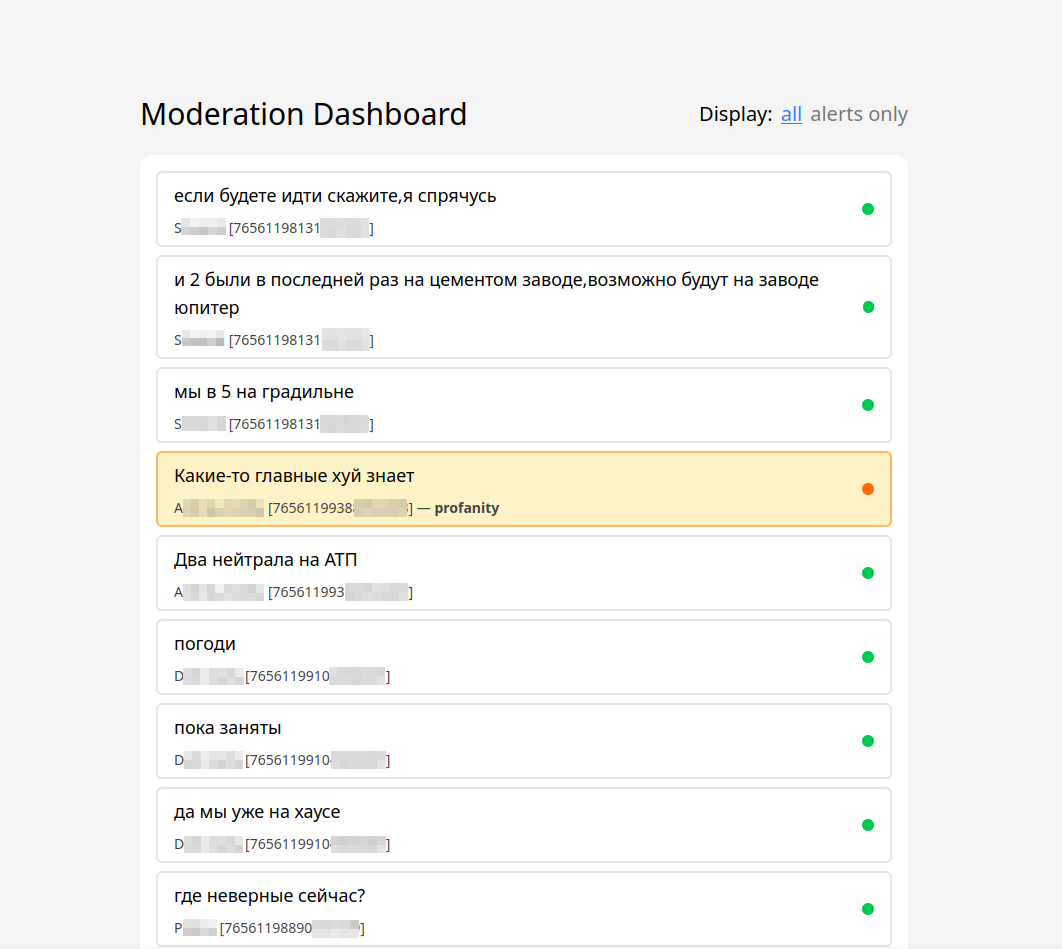
\includegraphics[width=0.9\textwidth]{dash-screenshot.png}
    \caption{Dashboard, seznam událostí}
    \label{fig:dashboard-main}
\end{figure}

Uživatelské rozhraní dashboardu tvoří webová stránka zobrazující seznam zpráv, které byly zpracovány systémem pro detekci toxicity. Hlavní část rozhraní tvoří svislý seznam zpráv, přičemž u každé položky je uveden text zprávy, jméno odesílatele včetně identifikátoru a výsledek detekce.

V horní části rozhraní je umístěn ovládací prvek, který umožňuje přepínat mezi zobrazením všech zpráv a pouze zpráv označených jako toxické. Každá zpráva je doplněna barevným indikátorem: zelená tečka označuje netoxickou zprávu, oranžová tečka značí zprávu detekovanou jako toxickou. U toxických zpráv je navíc uvedena rozpoznaná kategorie, například „profanity“.

Stránka obsahuje nadpis a umožňuje automatickou aktualizaci zobrazovaných dat v závislosti na příchozích událostech. Informace jsou rozčleněny do oddělených bloků, což podporuje orientaci v zobrazovaném obsahu.

\section{Implementace}

Dashboard tohoto systému je realizován jako webová aplikace s využitím frameworku Svelte a jazyka TypeScript. Jeho hlavní funkcí je zobrazování zpráv zpracovaných systémem detekce toxicity v téměř reálném čase. Komunikace mezi dashboardem a backendem probíhá prostřednictvím API, které poskytuje detekční události ve formátu JSON.

Detekční události vznikají na základě činnosti moderátorského bota pro Discord, který analyzuje zprávy a pro každou z nich vytvoří záznam. Tento záznam obsahuje jméno a identifikátor odesílatele, obsah zprávy, výsledek detekce toxicity a případně přiřazenou kategorii nebo důvod pro označení zprávy jako toxické. Události jsou serializovány do formátu JSON a ukládány do in-memory databáze Redis. Tyto záznamy jsou uchovávány ve tříděném seznamu podle časového razítka, což umožňuje efektivní získání nejnovějších zpráv a odstraňování zastaralých dat.

Dashboard periodicky načítá nové události z backendového API a aktualizuje zobrazení při dostupnosti nových dat. Uživatelské rozhraní rozlišuje mezi toxickými a běžnými zprávami pomocí vizuálního zvýraznění. Je možné filtrovat zobrazené události a zobrazit buď všechny zprávy, nebo pouze ty označené jako toxické. Pro každou událost jsou zobrazeny informace o odesílateli pro snadnější dohledatelnost.

Dashboard je navržen tak, aby informace zobrazoval v přehledné a strukturované podobě a napomáhal tak při moderaci zpráv v prostředí Discordu. Jeho implementace umožňuje přizpůsobení požadavkům konkrétního moderátorského workflow.

\chapter*{Závěr}
\addcontentsline{toc}{chapter}{Závěr}

Tento  projekt si kladl za cíl navrhnout a implementovat nástroj pro automatickou detekci toxických zpráv na platformě Discord, který by sloužil jako pomocný prostředek pro moderaci komunitních herních serverů. Projekt vycházel z reálného problému správy dvou komunitních serverů – Nullhaven (pro Minecraft) a Kill or Die Stalker RP (pro DayZ), které aktivně využívají Discord jako hlavní komunikační platformu mezi hráči, správci i moderátory.

Bezpečnostní politika Discordu je velmi přísná, zejména co se týče výskytu nenávistného, toxického nebo jinak nevhodného obsahu. I krátkodobé porušení pravidel ze strany uživatelů může vést k dočasnému nebo trvalému zablokování Discord serveru. Pokud takový server slouží pro komunitu s aktivními mikrotransakcemi nebo placeným obsahem, znamená to přímé komerční riziko a potenciální finanční ztráty. Manuální moderace tisíců zpráv denně je prakticky nemožná – právě zde přichází na řadu automatizace.

Nejprve jsme vytvořili skript, který prostřednictvím přímého přístupu k Discord API automaticky stahuje zprávy z vybraných kanálů. Struktura zpráv se lišila podle typu kanálu (osobní nebo veřejný), a proto jsme vyvinuli vlastní systém pro detekci a parsování každého typu zvlášť. Během sběru jsme nashromáždili přes 10 000 reálných zpráv.

Každá zpráva byla následně ručně anotována jako „normální“ (0) nebo „toxická“ (1). Vzhledem k tomu, že většina zpráv byla v azbuce, byla přidána automatická transliterace do latinky pro kompatibilitu s některými NLP nástroji. Přesto zůstala podpora pro práci s cyrilicí.

Testovali jsme a porovnali čtyři různé přístupy k detekci:

\begin{itemize}
    \item Regex filtrace: založená na slovníku vulgarismů a pravidelných výrazů.
    \item Předtrénovaný ruBERT-toxic: model trénovaný na obecném ruském datasetu s toxickým obsahem.
    \item Náš vlastní ruBERT: natrénovaný na našem datasetu přímo z Discord zpráv.
    \item LLM (Velký jazykový model): např. model běžící na platformě Groq, který umožňuje kontextovou analýzu zpráv.
\end{itemize}

Výsledky byly statisticky vyhodnoceny pomocí klasifikačních metrik (accuracy, precision, recall, F1-score). Nejslabších výsledků dosáhl regex filtr (F1-score = 0,61), nejlepších pak náš vlastní ruBERT model (F1-score = 0,95). Výsledky byly přehledně uvedeny v tabulkách s komentáři.

Kromě vytvoření modelu jsme navrhli i systém reálného sledování zpráv. V rámci Python skriptu je možné:

\begin{itemize}
    \item v reálném čase sledovat přicházející zprávy z Discord kanálů,
    \item automaticky je klasifikovat jako „normální“ nebo „toxické“,
    \item ukládat výsledek do souboru pro audit nebo zpětnou kontrolu,
    \item zobrazovat výstup v konzoli i jako log.
\end{itemize}

Součástí řešení je i nasazení LLM modelu (např. Groq) do webového dashboardu, který umožňuje:

\begin{itemize}
    \item zadávat zprávy ručně a získat predikci včetně důvěry,
    \item zobrazit historii analýz,
    \item využít LLM k detailnímu jazykovému rozboru a predikci v hraničních případech.
\end{itemize}
Díky této integraci máme k dispozici plně interaktivní prostředí pro moderátory i správce komunitních serverů.

Realizovaný systém představuje funkční a efektivní řešení pro automatickou moderaci zpráv. Spojením reálného datasetu, moderních jazykových modelů a automatizovaného sběru dat se podařilo vytvořit nástroj, který nejen snižuje nároky na lidské moderátory, ale zároveň zvyšuje bezpečnost a kvalitu komunikace v online komunitách.

Tento projekt zároveň ukázal, jak lze využít techniky z oblasti NLP a strojového učení v praktickém kontextu a připravil základ pro budoucí rozšíření – například nasazení plně automatického bota pro mazání nebo blokaci zpráv v reálném čase.

\printbibliography[title={Použitá literatura}, heading=bibintoc]

\end{document}
